\documentclass [14 pt]{article}
\usepackage[a4paper, total={6in, 8in}]{geometry}

\usepackage{fancyhdr}

\usepackage{hyperref}
\usepackage{graphicx}
\usepackage{float}
\usepackage{color}
\usepackage[english]{babel}
\usepackage[utf8]{inputenc}
\usepackage{listings}
\usepackage{multicol}
\usepackage{subcaption}
\usepackage{caption}
\usepackage{multirow}
\usepackage{titling}
\renewcommand\maketitlehooka{\vfill}
\renewcommand\maketitlehookd{\vfill\null}

\definecolor{deepblue}{rgb}{0,0,0.5}
\definecolor{deepred}{rgb}{0.6,0,0}
\definecolor{deepgreen}{rgb}{0,0.5,0}

\lstset{
language=Python,
	belowcaptionskip=1\baselineskip,
  	frame=single,
  	numbers=left,
  	xleftmargin=\parindent,
  	basicstyle=\ttfamily\scriptsize,
  	showspaces=false,
  	showtabs=false,
 	breaklines=true,
  	showstringspaces=false,
  	breakatwhitespace=false,
    keywordstyle=\color{deepblue},
    stringstyle=\color{deepgreen},
    rulecolor= \color{black},
}

\linespread{1.25}

\title{Project 1: Bad Smell Detection}
\author{Ardig\`o Susanna}
\begin{document}

\pagestyle{fancy}
\fancyhf{}
\lhead{Ardig\`o Susanna}
\rhead{Knowledge Analysis \& Management}
\cfoot{\thepage}

\begin{titlingpage}
\maketitle
\centering
\url{https://github.com/SusyPinkBash/bad_smell_detection}
\end{titlingpage}

\newpage\thispagestyle{plain}
\tableofcontents
\newpage

\section{Ontology Creation} % 1: intro
\subsection{Goal and Input parameter}
This part of the project consists of creating an ontology for Java Entities.\\
This file takes an optional argument which is the path of the python file that defines the Java Abstract Syntax Tree. If the argument is non supplied then a predefined path is used. For this project we used the file \texttt{tree.py} of the \href{https://github.com/c2nes/javalang}{Javalang} Python Library. 

\subsection{Description of the code}
In order to efficiently parse this file we created a class named \texttt{Class} to store the name, superclasses and properties of each class.
The function \texttt{get\_classes(python\_file\_name)} reads the given file, parses into an Abstract Syntax Tree. We use the function \texttt{walk} to iterate the tree, create instances of \texttt{Class} with the class definition nodes and save them into an array.\\
The main function \texttt{start} creates an ontology using the library \href{https://pythonhosted.org/Owlready2/}{Owlready2}. We then iterate the list of the parsed classes to create them in the ontology. This step needs to differentiate among three different contructions depending on the number of superclasses.
If the current class has none, meaning that it has no super class, in the ontology it is created as a subclass of Thing which, in owl, is the top superclass of all classes.
If the current class has one superclass, it is created as its subclass.
If the current class has two superclass, it is created as subclass of both.\\
For each class we add the previously extracted properties and add them to the ontology. There are two different types: 
Object, which are only \texttt{body} and \texttt{parameters}, and Data, which are all other properties.
Since the first type has only two possible values, we decided to add them only once at the end. To avoid conflict, when we create "name" properties we rename them to "jname".\\
The ontology is finally created and we can export it into an owl file.

\subsection{Results}
% 1: results
Figure \ref{fig:OntoClassGraph} shows the hierarchy tree of the created classes and properties, table \ref{tab:Population} shows their count.\\
We can see that \texttt{Statement} is the biggest superclass with 15 subclasses. The second biggest hierarchy is \texttt{Expression} with 8 direct subclasses some of which are superclasses themselves, with a total of 15 extra subclasses. \texttt{Documented} and \texttt{Declaration} share some subclasses.

% table
\begin{table}[h]
\centering
\begin{tabular}{| l r |}
\hline
\textbf{Type}		&  \textbf{\#}	\\ \hline\hline
Class	 			&	78	\\
Object Property		&	2	\\
Data Property		&	65	\\ \hline
\hline
\end{tabular}
\captionof{table}{Count of created classes and properties}\label{tab:Population}
\end{table}

% image
\begin{figure}[H]
\centering
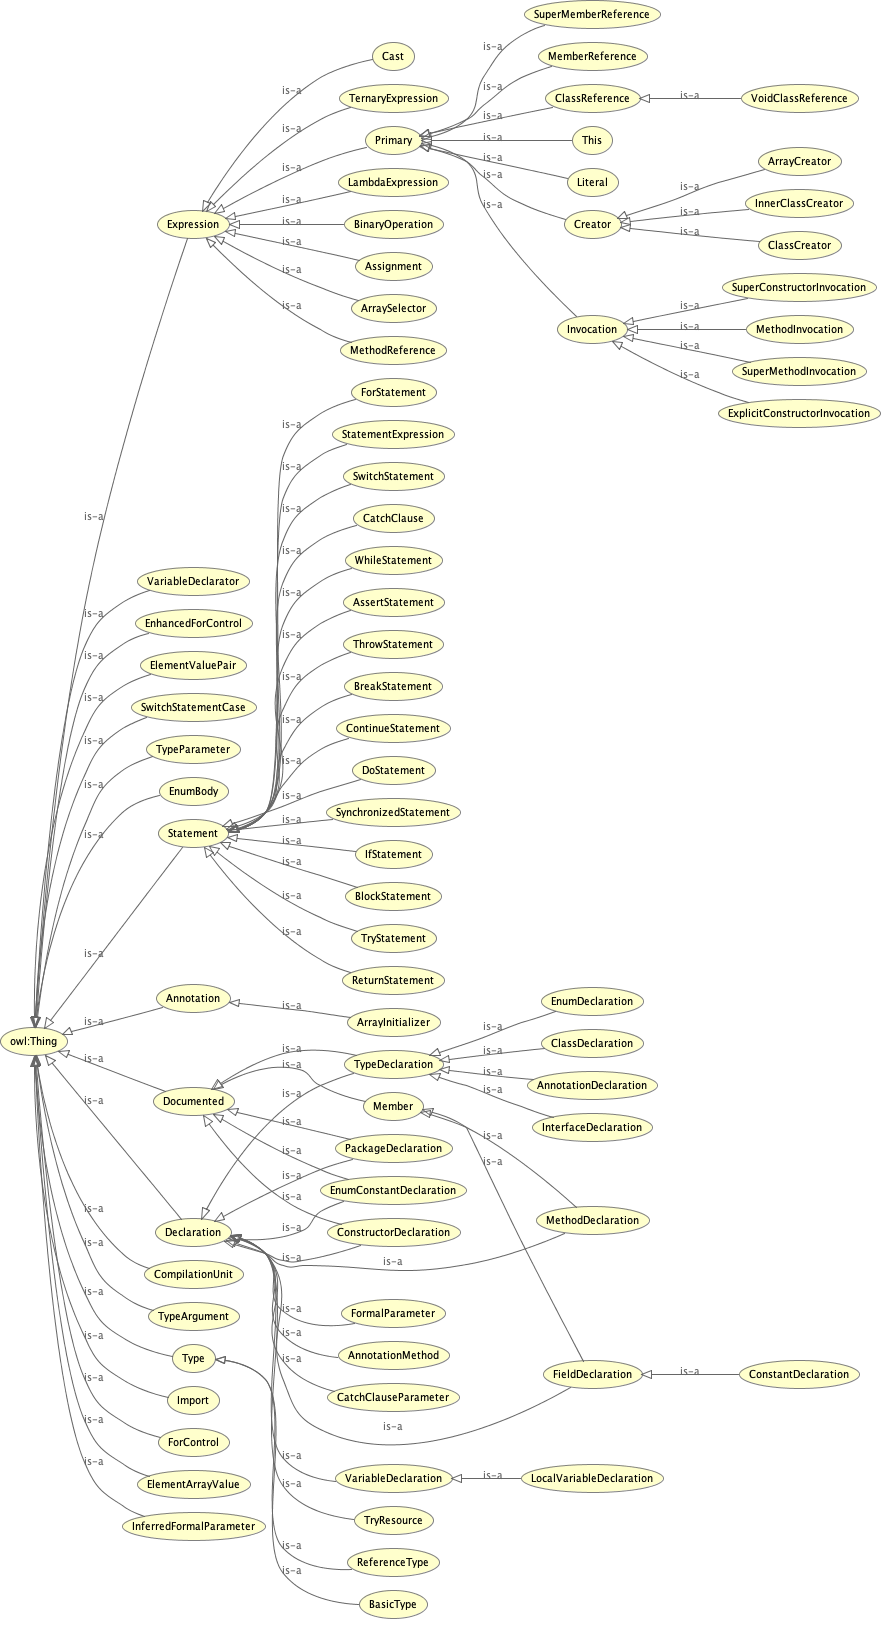
\includegraphics[height=0.9\textheight]{res/ontology_graph.png}
\caption{Class Hierarchy of the Ontology created}\label{fig:OntoClassGraph}
\end{figure}


\newpage
\section{Populate the Ontology}
% 2: intro
\subsection{Goal and input parameters}
This part of the project consists in populating the previously created ontology with instances of \texttt{ClassDeclaration}, \texttt{MethodDeclaration}, \texttt{FieldDeclaration}, \texttt{Statements} (including its subclasses) and \texttt{FormalParameter}.
 .\\
This file takes as input the path of the folder containing the java files that we want to analyze. In this project we used the folder \texttt{res/android-chess/app/src/main/java/jwtc/chess/} of the project \texttt{android-chess} which has 11 classes in 9 java files. 

\subsection{Description of the code}
% 2: explanation
Before we can start we need to load the ontology created in the previous step. In the first part we used the standard library \texttt{os} to list the files in the given directory and filtered the result on the extension to only open java files. We then use the function \texttt{parse.parse} of the \href{https://github.com/c2nes/javalang}{Javalang} Python Library to parse the content into an Abstract Syntax Tree. I decided to save all the trees, checking that are \texttt{ClassDeclaration}s into a default dictionary to allow duplicates multiple classes with the same name.\\
For each class we create a \texttt{ClassDeclaration} instance in the ontology with the class name. We then iterate through its methods and create a new instance of \texttt{MethodDeclaration} with the method name and add it to the class declaration. We add \texttt{FormalParameter} declarations for all the parameters of the method. Its body contains all the statements which we use to create an instance in the ontology taking the statement type for the tree.
After the constructor we check the fields and create a \texttt{FieldDeclaration} for each.
As the Constructor is a particular method, its logic only differers in type of declaration which is \texttt{ConstructorDeclaration}. \\
At last we can save the newly created instances in an owl file.

\subsection{Results}
% 2: results
We found 1344 instances. 
Table \ref{tab:Population} shows statistics for the individuals created for the considered project directory.

\begin{table}[H]
\centering
\begin{tabular}{| l r |}
\hline
\textbf{Class}			&  \textbf{\#}	\\ \hline\hline
ClassDeclaration 		&	11	\\
ConstructorDeclaration	&	6	\\
MethodDeclaration		&	152	\\
FieldDeclaration		&	105	\\
FormalParameter			&	165	\\ \hline
AssertStatement			&	0	\\ 
BlockStatement			&	143	\\ 
BreakStatement			&	23	\\ 
CatchClause				&	8	\\ 
ContinueStatement		&	4	\\ 
DoStatement				&	2	\\
ForStatement				&	6	\\
IfStatement				&	125	\\
ReturnStatement			&	106	\\
StatementExpression		&	446	\\
SwitchStatement			&	8	\\
SynchronizedStatement	&	1	\\
ThrowStatement			&	15	\\
TryStatement				&	8	\\
WhileStatement			&	10	\\ \hline
\hline
\end{tabular}
\captionof{table}{Number of created instances per class}\label{tab:Population}
\end{table}

\newpage
\section{Find Bad Smell}
\subsection{Goal and input parameters}
% 3: intro
This last part of the project consists of finding bad smells in the Java classes previously parsed into ontology individuals.\\
In order to find bad smells we execute \href{https://rdflib.readthedocs.io/en/stable/apidocs/rdflib.plugins.sparql.html}{SparQL} queries in our ontology.\\
This file takes an optional argument which is the path of the owl file previously created. If the argument is non supplied then a predefined path is used.

\subsection{Description of the code}
% 3: explanation
Before we can start we need to create a graph to be able to execute the queries. We create a world, load the ontology created in the previous steps and get the graph.\\
In order to efficiently parse the code smells we created two class named, respectively, \texttt{ClassSmell} and \texttt{MethodSmell} to store the name of the class, the occurrences and, in the second one, the name of the method.
There are five different types of code smells which require five different queries:
\begin{itemize}
	\item LongMethod and LongConstructors: methods and constructors that have  20 or more statements.
	\item LargeClass: classes that have 10 or more methods
	\item MethodWithSwitch, ConstructorWithSwitch: methods and constructors that have switch statements.
	\item MethodWithLongParameterList, ConstructorWithLongParameterList: methods and constructors that have 5 or more parameters
	\item DataClass: classes that have only setters and getters.
\end{itemize}

We have created a function for each type of query: \texttt{query\_long}, \texttt{query\_large\_class}, \texttt{query\_with\_switch}, \texttt{query\_with\_long\_parameter\_list}. All these functions require the graph ad input. The functions that query both methods and constructors take as input also the type of query.
These query functions are straight forward: in the first lines there is the query string, we run the query, filter the result based on a threshold described above and return an array with instances of \texttt{ClassSmell} of \texttt{MethodSmell} depending on the type of query. The results of all queries is then saved into a dictionay with the code smell name as a key.
The function \texttt{prepare\_query} is used to initialize the namespace of the queries. We created a function to print the results on the console.
\subsection{Results}
% 3: results
Table \ref{tab:BadSmellResults} shows the number of occurrences of each bad smell found in the code.\\
We can see that the constructors do not have any bad smells, there is only data class and the main bad smell is long methods.
I created different tables to show the results found for each query:
table \ref{tab:LongMethod} reports the results of LongMethod,
table \ref{tab:LargeClass} reports the results of LargeClass,
table \ref{tab:MethodWithSwitch} reports the results of LongMethod,
table \ref{tab:MethodWithLongParameterList} reports the results of MethodWithLongParameterList,
table \ref{tab:DataClass} reports the results of DataClass.
\begin{table}[h]
\centering
\begin{tabular}{|l  r|}
\hline	\textbf{Query}				&  \textbf{\#}	\\ \hline\hline
LongMethod							&	10	\\ 
LongConstructor						&	0	\\ 
LargeClass							&	3	\\ 
MethodWithSwitch					&	8	\\ 
ConstructorWithSwitch				&	0	\\ 
MethodWithLongParameterList			&	4	\\ 
ConstructorWithLongParameterList	&	0	\\ 
DataClass							&	1	\\ \hline
\end{tabular}
\captionof{table}{Bad smells (total)}\label{tab:BadSmellResults}
\end{table}


% LongMethod
\begin{table}[h]
\centering
\begin{tabular}{|l  l r|}
\hline
\textbf{Class}		&  \textbf{Method}	&  \textbf{\# of statements}	\\ \hline\hline
PGNProvider 			&	insert				&	31	\\ \hline
\multirow{2}{*}{ChessPuzzleProvider}
	&	query				&	25	\\
	&	insert				&	20	\\ \hline
\multirow{4}{*}{GameControl}
	&	loadPGNHead			&	26	\\
	&	loadPGNMoves		&	96	\\
	&	requestMove			&	76	\\
	&	getDate				&	26	\\ \hline
\multirow{3}{*}{JNI}
	&	newGame				&	35	\\
	&	initFEN				&	88	\\
	&	initRandomFisher	&	87	\\ \hline
\end{tabular}
\captionof{table}{Long methods}\label{tab:LongMethod}
\end{table}

% LargeClass
\begin{table}[h]
\centering
\begin{tabular}{|l  r|}
\hline
\textbf{Class}		&  \textbf{\# of methods}	\\ \hline\hline
GameControl 			&	63	\\
JNI		 			&	44	\\
Move	 			&	21	\\
\hline
\end{tabular}
\captionof{table}{Large class}\label{tab:LargeClass}
\end{table}

% MethodWithSwitch
\begin{table}[h]
\centering
\begin{tabular}{|l  l r|}
\hline
\textbf{Class}		&  \textbf{Method}	&  \textbf{\# of switch}	\\ \hline\hline
\multirow{4}{*}{PGNProvider}
	&	query				&	1	\\
	&	getType				&	1	\\ 
	&	delete				&	1	\\ 
	&	update				&	1	\\ \hline
\multirow{4}{*}{ChessPuzzleProvider}
	&	query				&	1	\\
	&	getType				&	1	\\ 
	&	delete				&	1	\\ 
	&	update				&	1	\\ \hline
\end{tabular}
\captionof{table}{Methods with switches}\label{tab:MethodWithSwitch}
\end{table}


% MethodWithLongParameterList
\begin{table}[H]
\centering
\begin{tabular}{|l  l r|}
\hline
\textbf{Class}		&  \textbf{Method}	&  \textbf{\# of parameters}	\\ \hline\hline
PGNProvider			&	query				&	5	\\ \hline
ChessPuzzleProvider	&	query				&	5	\\ \hline
GameControl			&	addPGNEntry			&	5	\\ \hline
JNI					&	setCastlingsEPAnd50	&	6	\\ \hline
\end{tabular}
\captionof{table}{MethodWithLongParameterList query results}\label{tab:MethodWithLongParameterList}
\end{table}

% DataClass
\begin{table}[H]
\centering
\begin{tabular}{|l  r|}
\hline
\textbf{Class}		&  \textbf{\# of methods}	\\ \hline\hline
Valuation 			&	1	\\
\hline
\end{tabular}
\captionof{table}{Data classes}\label{tab:DataClass}
\end{table}


\newpage
\appendix

\section{Python code}

\subsection{Project}
\subsubsection{Create Ontology}
\lstinputlisting{../src/onto_creator/onto_creator.py}
\subsubsection{Populate Ontology}
\lstinputlisting{../src/individ_creator/individ_creator.py}
\subsubsection{Find Bad Smell}
\lstinputlisting{../src/bad_smells/bad_smells.py}

\subsection{Tests}
\subsubsection{Create Ontology}
\lstinputlisting{../src/onto_creator/onto_creator_tests.py}
\subsubsection{Populate Ontology}
\lstinputlisting{../src/individ_creator/individ_creator_tests.py}
\subsubsection{Find Bad Smell}
\lstinputlisting{../src/bad_smells/bad_smells_tests.py}



\section{Bash Code} 
\subsection{Run Project}
\lstinputlisting[language=Bash]{../run.sh}
\subsection{Test Project}
\lstinputlisting[language=Bash]{../test.sh}


\end{document}